\begin{figure}[H]
\centering
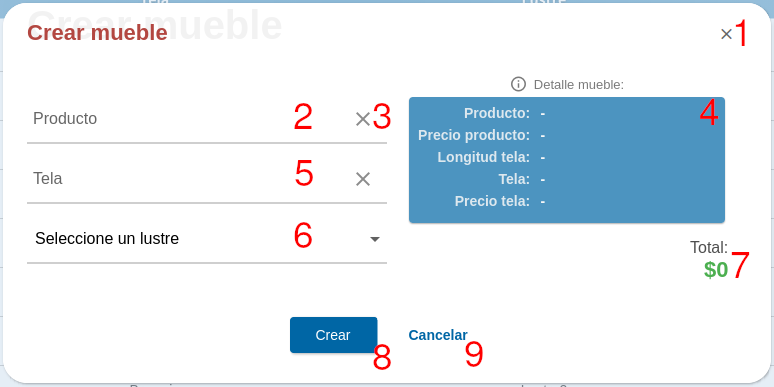
\includegraphics[width=\textwidth,height=\textheight,keepaspectratio]{Escenarios/AD-49-00}
\caption{Escenario - AD-49-00}
\label{fig:AD-49-00}
\end{figure}

Este escenario permite a un usuario crear un mueble, con el botón \textbf{AD-49-01} se podrá cerrar la ventana y volver al escenario \textbf{AD-48-00}.
El usuario debe ingresar el nombre de un producto en el campo \textbf{AD-49-02} y de una tela en el campo \textbf{AD-49-05} desplegándose un menú de opciones en cada caso con productos y telas existentes respectivamente. También si hace click en el campo \textbf{AD-49-06} se desplegará un menú con opciones de lustres existentes para que seleccione uno. 
Si el usuario hace click en el botón \textbf{AD-49-03} podrá borrar lo que haya ingresado en el campo correspondiente, en este caso el campo \textbf{AD-49-02}. 
Si el usuario hace click en el botón \textbf{AD-49-08} creará el mueble de acuerdo a los campos ingresados y si hace click en el botón \textbf{AD-49-09} cancelará, cerrando la ventana y volviendo al escenario \textbf{AD-48-00}.
\\